%%
% 引言或背景
% 引言是论文正文的开端,应包括毕业论文选题的背景、目的和意义;对国内外研究现状和相关领域中已有的研究成果的简要评述;介绍本项研究工作研究设想、研究方法或实验设计、理论依据或实验基础;涉及范围和预期结果等。要求言简意赅,注意不要与摘要雷同或成为摘要的注解。
%%
% 章、节、小节、图片、公式、表格下方的\label{...}标记不建议删除,因为这些可以做到自动引用的作用,当某些公式、图片被删除时,\label{...}标记能使正文中的编号自动更新,省去一个一个编号的麻烦。

\chapter{绪论}
\label{cha:introduction}
\section{引言}
\label{sec:prologue}
引言是论文正文的开端,应包括毕业论文选题的背景、目的和意义;对国内外研究现状和相关领域中已有的研究成果的简要评述;介绍本项研究工作研究设想、研究方法或实验设计、理论依据或实验基础;涉及范围和预期结果等。要求言简意赅,注意不要与摘要雷同或成为摘要的注解。

\section{国内外研究现状和相关工作}
\label{sec:related_work}
对国内外研究现状和相关领域中已有的研究成果的简要评述。

\section{快速上手}
\label{sec:latex_basic}
本模板不会提及过多花里胡哨的操作,只追求使用者正确配置、快速上手使用LaTeX,拿到模板后即能专注于论文内容的撰写,不会纠结于配置以及其它有关代码的问题。下面介绍一种能成功配置的方法,是我使用的配置方法。

以下操作步骤均在Windows 10/11操作系统中完成,不建议在Linux系统中操作,因为Linux系统会涉及额外的字体安装、配置等问题,并且本人实测,同样是TeX Live编译,同样的文件,同一台电脑安装Ubuntu 20.04.3/Windows 11双系统,在Windows 10/11中编译生成pdf更快。

第一步,下载TeX Live并安装。建议从知名的开源镜像站下载安装包,如中科大开源镜像站(图 \ref{fig:ustc})、清华大学开源镜像站(图 \ref{fig:tsinghua})等,TeX Live一般在CTAN目录下(图 \ref{fig:texlive}),建议下载并安装2021及更新版本。
\begin{figure}[htbp] 
	\centering
	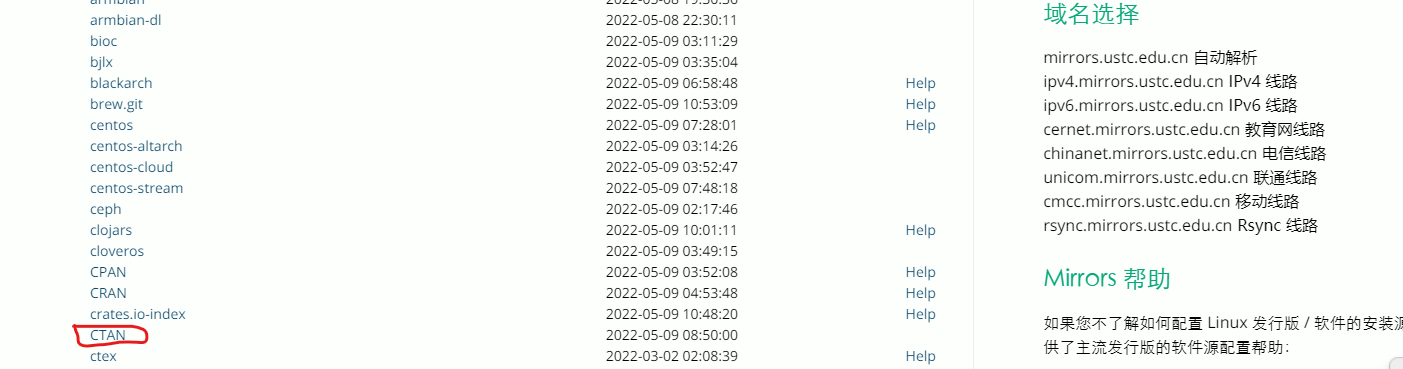
\includegraphics[width=0.85\textwidth]{image/chap01/ustc.png}
	\caption{中科大开源镜像站}
	\label{fig:ustc}
\end{figure}
\begin{figure}[htbp] 
	\centering
	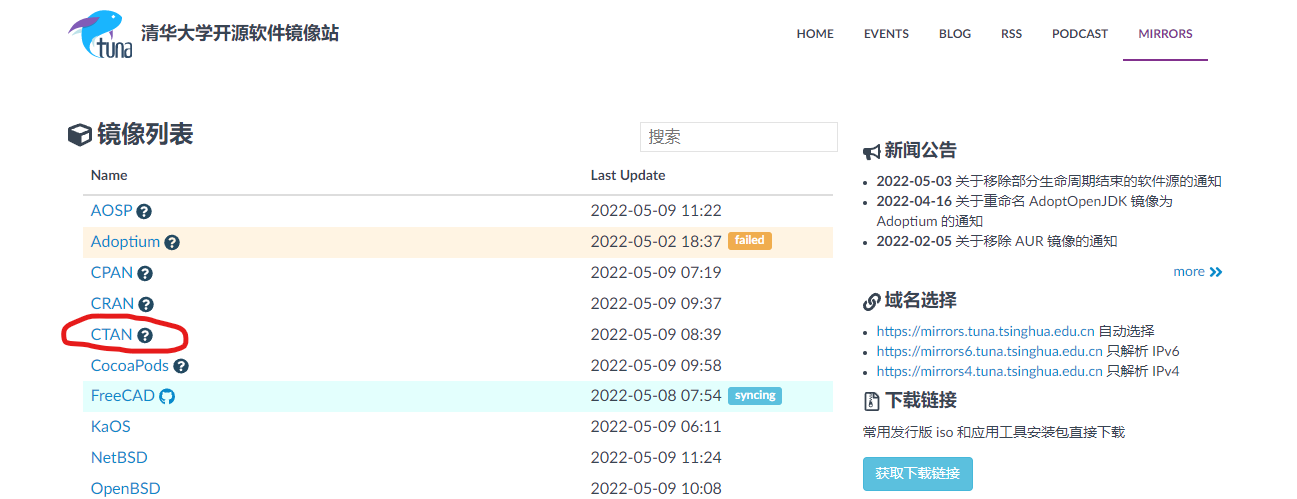
\includegraphics[width=0.85\textwidth]{image/chap01/tsinghua.png}
	\caption{清华大学开源镜像站}
	\label{fig:tsinghua}
\end{figure}
\begin{figure}[htbp] 
	\centering
	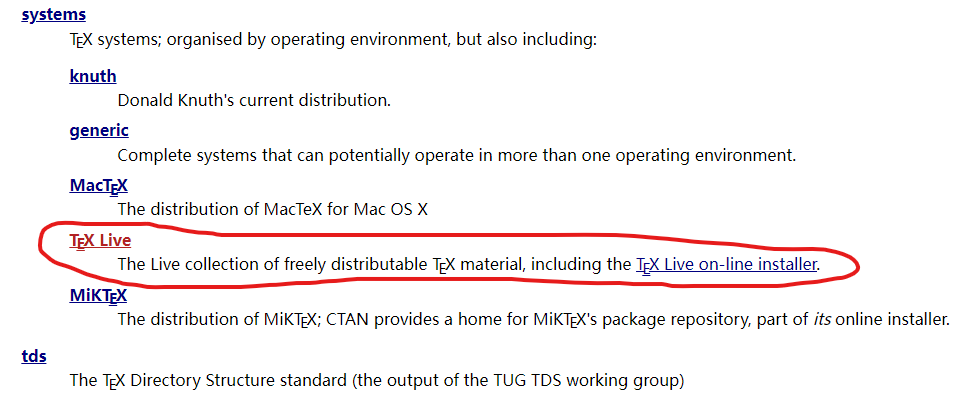
\includegraphics[width=0.7\textwidth]{image/chap01/texlive.png}
	\caption{texlive下载}
	\label{fig:texlive}
\end{figure}

%第二步,安装CTAN宏包。在开始菜单中找到Tex Live command-line(图 \ref{fig:texlivecmd}),以管理员模式运行,依次运行以下两行命令:

%\noindent tlmgr option repository http://mirrors.aliyun.com/CTAN/systems/texlive/tlnet/

%\noindent tlmgr update $ \text{-}\text{-} $self $ \text{-}\text{-} $all

%\noindent 等待CTAN宏包更新自动完成即可。
%\begin{figure}[htbp] 
	\centering
	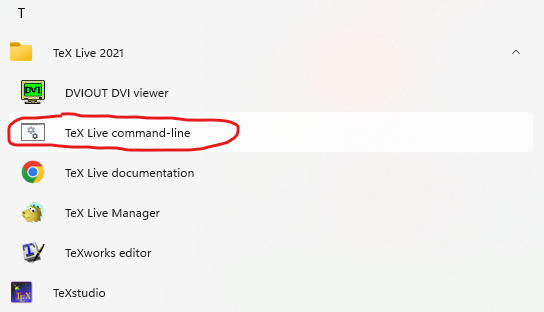
\includegraphics[width=0.6\textwidth]{image/chap01/texlivecmd.png}
	\caption{TeX Live command-line}
	\label{fig:texlivecmd}
\end{figure}

第二步,安装TeXstudio并配置。一般来说安装完成之后TeXstudio能自动识别已安装的TeX Live,打开TeXstudio,在上方找到Options $\rightarrow$ Configure TeXstudio并点击(图 \ref{fig:texstudio1}),在Build中将Default Compiler选为XeLaTeX,Default Bibliography Tool(默认参考文献工具)选为BibTeX(图 \ref{fig:texstudio2})。
\begin{figure}[htbp] 
	\centering
	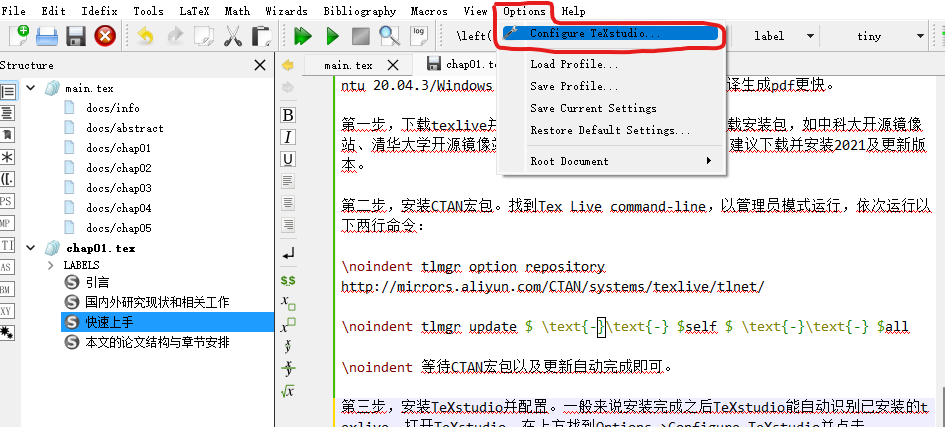
\includegraphics[width=1\textwidth]{image/chap01/texstudio1.png}
	\caption{TeXstudio Configure位置}
	\label{fig:texstudio1}
\end{figure}
\begin{figure}[htbp] 
	\centering
	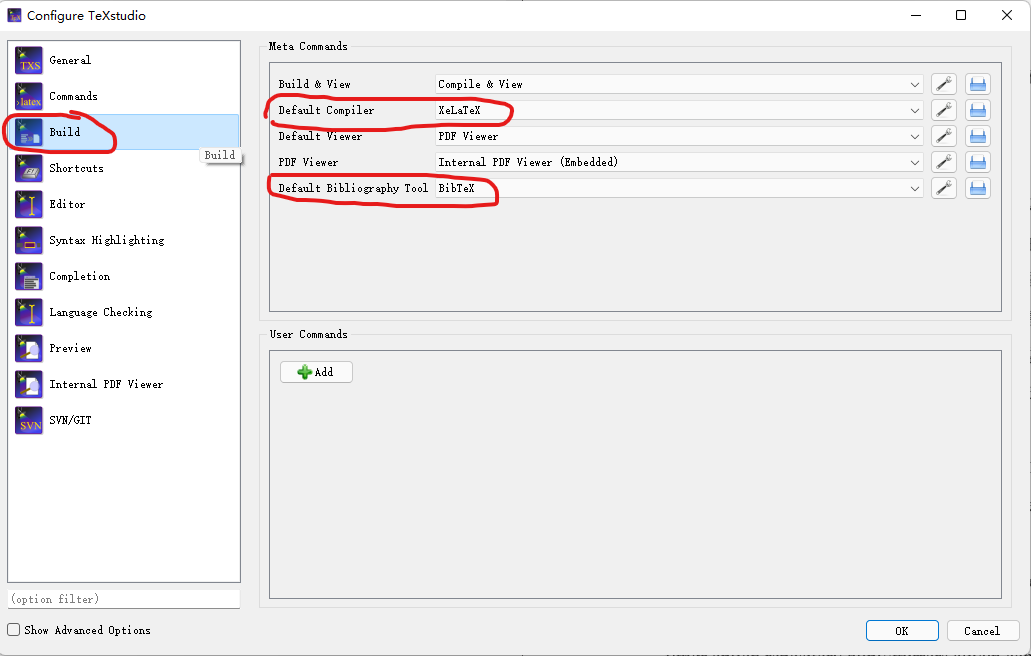
\includegraphics[width=1\textwidth]{image/chap01/texstudio2.png}
	\caption{TeXstudio Configure设置}
	\label{fig:texstudio2}
\end{figure}

第三步,编译生成pdf文档,操作为:用TeXstudio打开main.tex文件,点击上方绿色双箭头(Build \& View)(图 \ref{fig:f5}),等待LaTeX自动完成编译过程,就能生成正确的pdf文档。
\begin{figure}[H] 
	\centering
	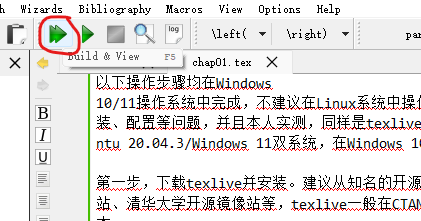
\includegraphics[width=0.6\textwidth]{image/chap01/f5.png}
	\caption{Build \& View}
	\label{fig:f5}
\end{figure}

综上,上述三个步骤的操作能让你在Windows 10/11+TeX Live+TeXstudio的环境下得到与github页面中内容一模一样的pdf文档。

\section{本文的论文结构与章节安排}
\label{sec:arrangement}
本文共分为五章,各章节内容安排如下:

第一章为绪论。

第二章为本模板遵循的排版及格式。

第三章为图像的插入示例。

第四章为公式与表格的插入示例

第五章是本文的最后一章,结论与展望。是对本文内容的整体性总结以及对未来工作的展望。

